% !TeX root = ../Notizen.tex

\section*{Aufgabe1: 2D Lennard-Jones Fluid}
\subsection*{Einleitung}
Es Wird eine Molekulardynamik Simulation für N=16 Teilchen geschrieben, die alle die Masse $m=1$ besitzen.
Das Verwendete Potential ist das Lennard-Jones Potential
\begin{align*}
	V_{LJ}(r)=4\left[ \left(\frac{1}{r}\right)^{12} - \left(\frac{1}{r}\right)^6\right]
\end{align*} 
Es wird ein Cutoff $r_c=L/2$ eingebaut, für dass Potential so dass 
\begin{align*}
	V_{c}=
	\begin{cases}
		V_{LJ}(r)-V_{LJ}(r_c)\text{ wenn }  r<r_c\\
		0 \text{  sonst}
	\end{cases}
\end{align*}
Die Kraft die daraus Folgt ist
\begin{align*}
	\vec{F}_{LJ}=
	\begin{cases}
		\frac{\vec{r}}{r}\frac{48}{r}\left[ \left(\frac{1}{r} \right)^{12}-\frac{1}{2}\left(\frac{1}{r}\right)^6\right] \text{ wenn } r < r_c\\
		0 \text{   sonst}
	\end{cases}
\end{align*}
und die Kraft die auf ein Teilchen $i$ wirkt ist demnach
\begin{align*}
	\vec{F}_i = \sum\limits_{j=1 , \atop i\not= j}^{N} \vec{F}_{LJ}\left( \vec{r}_i - \vec{r}_j \right).
\end{align*}
Weiter Wird in jeden Schritt die Energien und Temperaturen ausgerechnet.
\begin{align}
	E_{pot}&=\frac{1}{2}\sum\limits_{i=1 , \atop i\not= j}^{N} V_c \left(|r_i-r_j| \right),\\
	E_{kin}&=\sum\limits_{i=1}^{N}\frac{1}{2}m\vec{v}^2\\
	k_BT(t&)=\frac{2}{N_f}\sum\limits_{i=1}^{N}\frac{\vec{p}^2}{2m}= \frac{2}{N_f}\sum\limits_{i=1}^{N}\frac{1}{2}m\vec{v}^2
\end{align}
mit Anzahl der Freiheitsgrade $N_f=2N-2$ für 2 Dimensionen.
Genauso wird die Schwerpunktsgeschwindigkeit zu jeden Zeitpunkt bestimmt durch
\begin{align}
\vec{v}_s=\frac{1}{N}\sum\limits_{i=1}^{N}\vec{v}_i
\end{align}
Weiter wird noch die Definition einer zeitgemittelten Observablem $O$ benötigt
\begin{align}
\langle O \rangle_{MD} = \frac{1}{t_{md}}\sum\limits_{n=0}^{t_{MD}} O\left(\{\vec{r}(n\Delta t)\}, \ \{ \vec{p}(n\Delta t) \}\right)
\end{align}
\subsection*{a) Initialisierung}
Die Teilchen müssen zunächst eine Start Position und eine Start Geschwindigkeit bekommen.
Die Teilchen werden mithilfe von
\begin{align*}
\vec{r}(0)=\frac{1}{8}
\begin{pmatrix}
1+2n\\1+2m
\end{pmatrix}L
\end{align*}
angeordnet.
Die Geschwindigkeiten $v_{x,y}\in(-1,1)$ zufällig zugeordnet.
Die Schwerpunktsgeschwindigkeit soll verschwinden, dies wird erreicht in dem Von jeden Teilchen die Schwerpunktsgeschwindigkeit abgezogen wird.
Damit eine Temperatur im System eingestellt wird, wird die Geschwindikeit reskaliert mithilfe von
\begin{align}
	\alpha &= \sqrt{\frac{T_\text{eingestellt}}{T_\text{system}}}\\
	\vec{v}\ '&=\alpha\vec{v}.
\end{align}
\subsection*{Simulation}
Zur Lösung der Differentialgleichung für jedes Teilchen wird der Geschwindigkeits-Verlet-Algorithmus verwendet:
\begin{align*}
	\vec{r}(t_n)=&\vec{r}(t_{n-1})+\frac{1}{m}\vec{p}(t_{n-1})\Delta t + \frac{1}{2m}\vec{F}(t_{n-1})\Delta t^2\\
	\vec{p}(t_n)=&\vec{p}(t_{n-1}) + \left( \vec{F}(t_{n-1}) + \vec{F}(t_n) \right)\frac{\Delta t}{2}
\end{align*}
Dieser Algorithmus wurde gewählt, weil die Kraft nur ein mal aufgerufen werden muss pro Zeitschritt und Teilchen.
Dies hat den vorteil zu anderen Algorithmen das es zeitlich effizienter ist.
Weiter Sollen in dem System periodische Randbedingungen vorliegen.
Das heißt es gibt 8 weitere Abbilder von Urbild.
Die Positionen aller Bilder kann mithilfe von
\begin{align*}
	\vec{r}' = \vec{r}+L\vec{n}\\
	\vec{n}=
	\begin{pmatrix}
		n_x\\
		n_y
	\end{pmatrix}
\end{align*}
mit $n_i\in(-1,0,1)$.
Weiter müssen die Teilchen in dem Bereich bleiben des $L\times L$.
Dies wird durch
\begin{align*}
	x'=x-L\cdot \text{floor}(x/L)
	y'=y-L\cdot \text{floor}(y/L)
\end{align*}
\subsection*{b) Messung: Energie/Temperatur}
Das Programm gibt vier Dateien aus.
Eine in der die Postionen aller Teilchen gespeichert wird, zu jedem Zeitpunkt.
Eine in der $E_{pot},\ E_{kin},\ E_{ges},\ k_BT$ und $\vec{v}_s$ gespeichert wird, zu jeden Zeitpunkt.
Eine in der die Zeitgemittelten $\left<E_{kin}\right>,\ \left<E_{pot}\right>$ und $\left<T\right>$ gespeichert wird.
Zum Schluss wird eine Datei gespeichert in der die Paarverteilung $g(r)$ gespeichert wird.
\subsection*{Ergebnis}
Es werden Plots für die Konfiguration $L=4,0\sigma$, $T=1,0\epsilon$ und $\Delta t= 0,01s$ erstellt.
Aus \cref{fig:Energie_0} lässt sich erkennen,dass das System nach etwa 2 Sekunden äquilribriert.\\
\begin{figure}[h!]
	\centering
	\includegraphics[width = 0.5\textwidth]{../Plots/Plot_0_Orte.png}
	\caption{Die Teilchen Positionen in Änderung mit der Zeit, ist hier für alle 16 Teilchen dargestellt.}
\end{figure}

\begin{figure}[h!]
	\centering
	\includegraphics[width = 0.5\textwidth]{../Plots/Plot_0_Energie.pdf}
	\caption{Hier  sind für die Konfiguration die Energien dargestellt.}
\end{figure}

\begin{figure}[h!]
	\centering
	\includegraphics[width = 0.5\textwidth]{../Plots/Plot_0_Temperatur.pdf}
	\caption{Hier  sind für die Konfiguration die Temperatur dargestellt.}
\end{figure}

\begin{figure}[h!]
	\centering
	\includegraphics[width = 0.5\textwidth]{../Plots/Plot_0_schwer.pdf}
	\caption{Hier ist die Schwerpunktsgeschwindigkeit zu Erkennen, dabei ist drauf zu achten das die Y-Achse mit $10^{14}$ multipliziert wurde.}\label{fig:Energie_0}
\end{figure}

\begin{figure}[h!]
	\centering
	\includegraphics[width = 0.5\textwidth]{../Plots/Plot_0_E_OBS.pdf}
	\caption{Hier sind die Zeitgemittelten Energien dargestellt.}
\end{figure}\newpage

\subsection*{c) Paarverteilung}
Die Paarverteilung ist Definiert als
\begin{align*}
	\rho g^{(1)}(\vec{r}):=\left< \sum\limits_{i=1}^{N}\delta(\vec{r}-\vec{r_i})\right>
\end{align*}
mit $\rho=N/V$.
Gemessen wird die Paarverteilung mithilfe von Paarabständen.
Dazu wird das Intervall $0<r<L/2$ in $N_H$ Bins eingeteilt.
Daraus Folgt das jedes Bin die Breite $\delta r= L/2N_H$ besitzt.
Nun wird für jeden Zeitpunkt bestimmt wie viele Teilchen in dem Abstand $l\Delta r < |\vec{r}_i-\vec{r}_j<(l+1)\Delta r$ liegen, wobei $0\le l < N_H$.
Die Anzahl ist Proportional zum zeitgemittelten Druck $\langle p_l \rangle$.
Mit der Hilfe des Drucks kann $g(r_l)$ bestimmt werden.
\begin{align}
	g(r_l)=\frac{\langle p_l\rangle}{\Delta V\rho N}
\end{align}
Dabei ist $\Delta V$ das Volumen Element
\begin{align*}
	\Delta V \propto (l\Delta r)^2-((l-1)\Delta r)^2.
\end{align*}
Dadurch haben wir, eine Formel, die proportional zu $g(r)$ ist.
Es werden für drei Verschiedene Anfangstemperaturen $T_1(0)=1\epsilon,T_2(0)=0,01\epsilon$ und $T(0)=100\epsilon$ mit einer $L=8\sigma$, die Paarverteilungen bestimmt.
Dabei wird die Erst gemessen wenn das System äquilibert ist.
\begin{figure}[h!]
	\centering
	\subfigure[$\langle T_1(t)\rangle$]{\includegraphics[width = 0.49\textwidth]{../Plots/Plot_1_Temperatur_OBS.pdf}}
	\subfigure[$g(r)$]{\includegraphics[width = 0.49\textwidth]{../Plots/Plot_1_Paar.pdf}}
	\caption{Aus der Zeit gemittelten Temperatur, erkennt man dass das System ab $t=50s$ äquilibriert ist und aus dem Plot für die Paarverteilung lässt sich erkennen das ein Übergang zwischen fest vorliegt.}
\end{figure}
\begin{figure}[h!]
	\centering
	\subfigure[$\langle T_2(t)\rangle$]{\includegraphics[width = 0.49\textwidth]{../Plots/Plot_2_Temperatur_OBS.pdf}}
	\subfigure[$g(r)$]{\includegraphics[width = 0.49\textwidth]{../Plots/Plot_2_Paar.pdf}}
	\caption{Aus dem Plot der Temperatur $\langle T\rangle$ lässt sich erkennen, dass das System nach $60s$ äquilibriert ist. Aus dem Plot für die Paarkollerationsfunktion ist zu erkennen das es sich um eine flüssige Phase handelt.}
\end{figure}
\begin{figure}[h!]
	\centering
	\subfigure[$\langle T_3(t)\rangle$]{\includegraphics[width = 0.49\textwidth]{../Plots/Plot_3_Temperatur_OBS.pdf}}
	\subfigure[$g(r)$]{\includegraphics[width = 0.49\textwidth]{../Plots/Plot_3_Paar.pdf}}
	\caption{Aus dem Plot der Temperatur lässt sich erkennen, dass das System nach 20 Sekunden äquilibriert ist. Die Phase liegt im gasförmigen Bereich.}
\end{figure}\newpage
\subsection*{Thermostat}
Nun wird ein Thermostat ein gestellt, so das die Temperatur im System konstant bleibt.
Das geschieht wie bei der Initialisierung.
\begin{figure}[h!]
	\centering
	\subfigure[]{\includegraphics[width = 0.49\textwidth]{../Plots/Plot_D_Energie.pdf}}
	\subfigure[]{\includegraphics[width = 0.49\textwidth]{../Plots/Plot_D_Paar.pdf}}
	\centering
	\subfigure[]{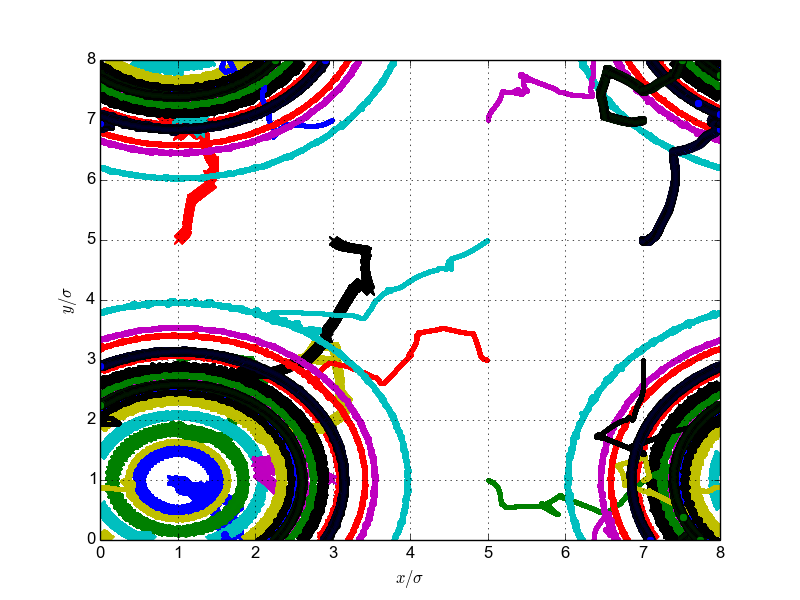
\includegraphics[width = 0.49\textwidth]{../Plots/Plot_D.png}}
	\subfigure[]{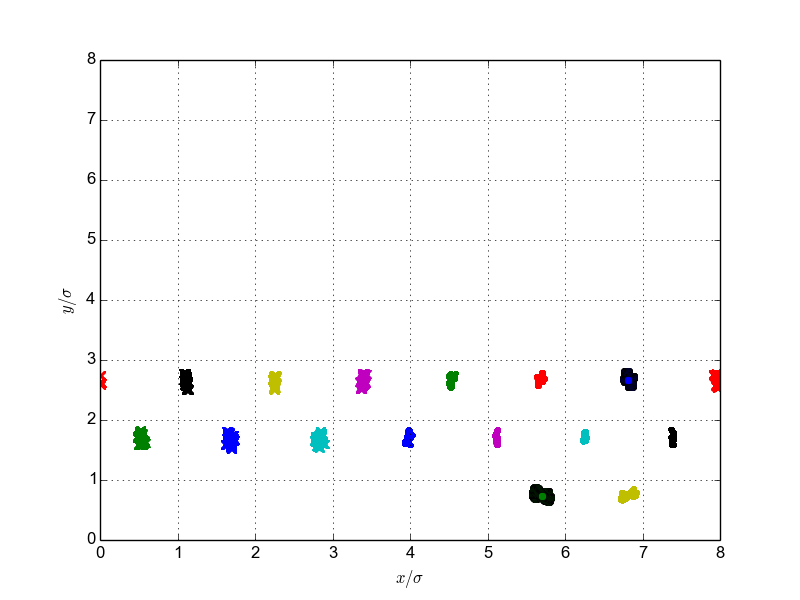
\includegraphics[width = 0.49\textwidth]{../Plots/Plot_D_1.png}}
\end{figure}